\begin{appendices}
%Material that is complementary to the main body of the report can be included in an appendix. For externally sponsored students, if a report has been submitted to the sponsor during the year of the review, the report should be included in the appendix (a copy of the report can be supplied by the PGR coordinator). The appendix should include a list of training courses (including dates, duration, etc.) taken by the student during the year and other relevant research activities such as given seminars, attendance and presentations to conferences, etc. The appendix could also include material that is supplementary to the main body of the report such as: description of data sets, detailed experimental results, papers that have been submitted or published, etc.

\chapter{Training Courses}
\begin{itemize}
\item Computer Science PGR Introductory Seminar 5 Dates
\item Tradition of Critique Lecture series, Monday 29th September - Monday 8th December (18:00 - 20:00)
\item Graduate School: 
	\begin{itemize}	
		\item Nature of the doctorate and the supervision process, 15th November 2016 (9:30 - 12:00)
		\item Presentation skills for researchers (all disciplines), 27th Jan 2017 (9:30 - 15:30)
		\item Planning your research, 20th Feb 2017 (9:30 - 13:00)
		\item Getting into the habit of writing, 23th Feb 2017 (9:30 - 12:30)
	\end{itemize}
\item Midland Graduate School 2017 from 9-13 April in Leicester. Attended courses on Denotational Semantics, Naïve Type Theory and Testing with Theorem Provers.
\end{itemize}

\chapter{Update-Strategies}
TODO: write short explanation of this paper: tries to develop foundational technical vocabulary for ABS.

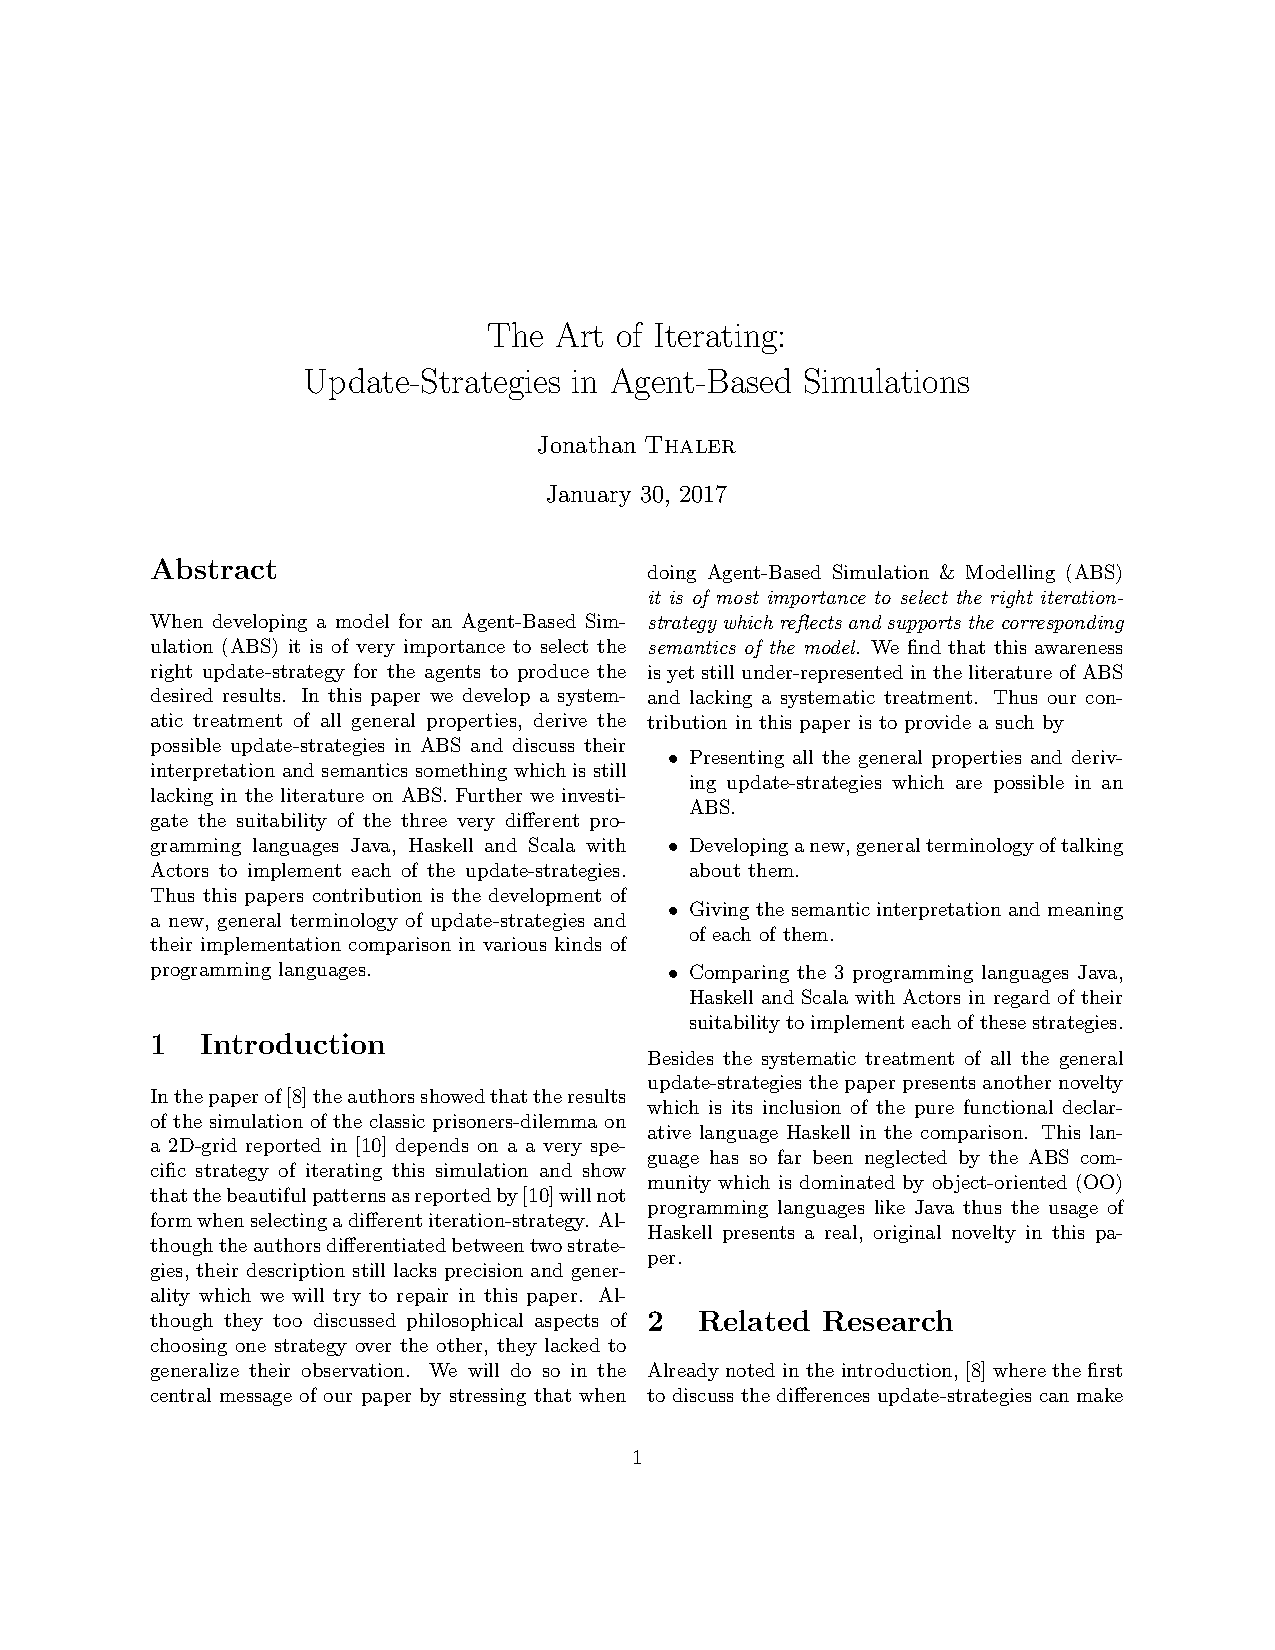
\includepdf[pages=-]{./pdf/iteratingABM.pdf}

\chapter{Programming-paradigms in ABS}
TODO: write short explanation of this paper. emphasize that it was not published but originally part of the update-strategies paper which was then split because of two different things mixed up.

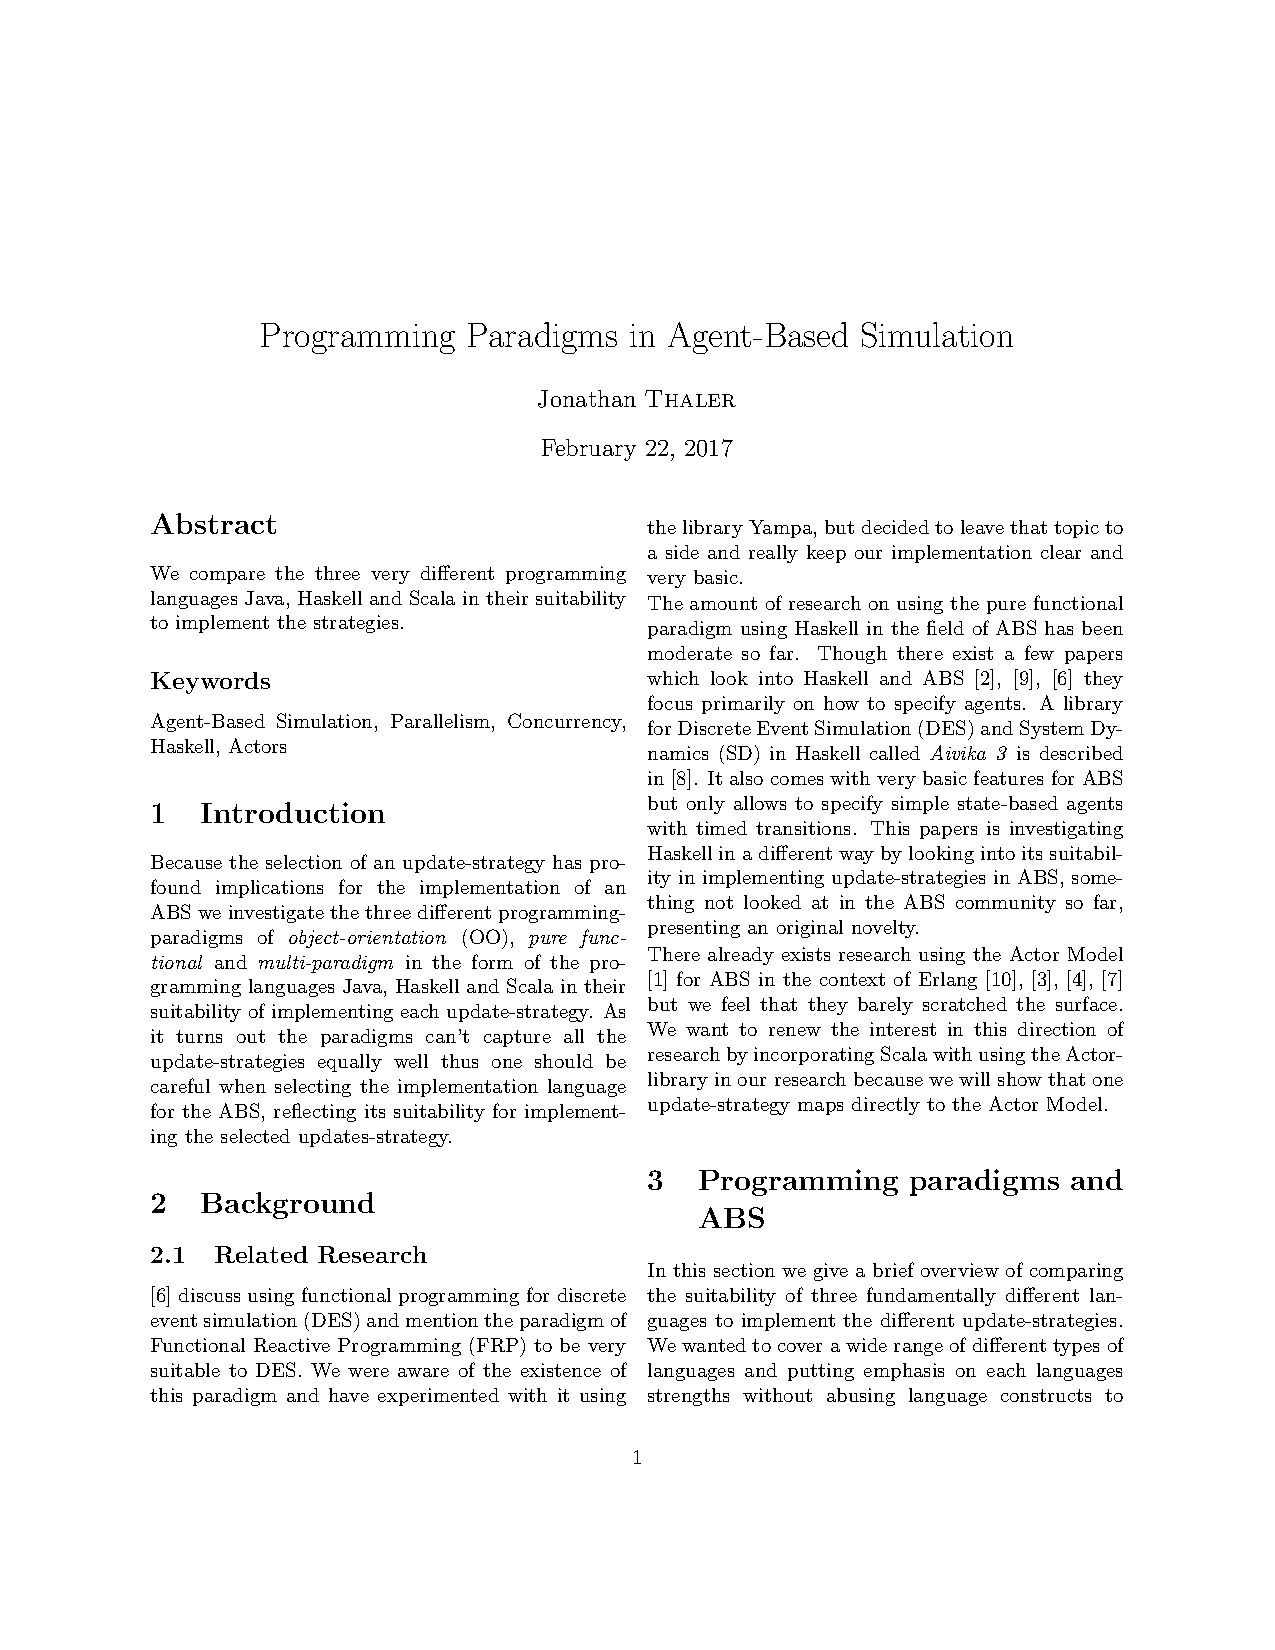
\includepdf[pages=-]{./pdf/programmingParadigmsABS.pdf}

\chapter{Recursive ABS}
TODO: write short explanation of this paper. not published but interesting idea but not enough time to pursue. also why stopped working: don't have the right model in which it serves as a killer-features. still we are convinced that it proves one of the major benefits of FrABS: recursion is easy to implement because the language is built on it and due to the lack of side-effects.

TODO: include, need little bit of refinement

\end{appendices}